% Section: Cross-Correlation Time Reconstruction (CC) and Out-of-Time Pile-Up Mitigation
\section{Cross-Correlation Time Reconstruction and Out-of-Time Pile-Up Mitigation}

The KUCC algorithm leverages out-of-time (OOT) pulse amplitudes determined by the multi-fit algorithm for rechit energy reconstruction to perform precise time reconstruction. Given these amplitudes and the known pulse shape of an isolated signal in a crystal, the nominal pulse contribution is reconstructed for each rechit. The cross-correlation (CC) method then determines the time by finding the best match between the extracted signal amplitudes and the pulse shape template. This procedure significantly mitigates the impact of OOT pile-up and improves the ECAL time resolution.

OOT-PU arises when signals from interactions in preceding or subsequent bunch crossings (BXs) overlap with the current BX. Since scintillation light in ECAL crystals has a decay longer than 25 ns, signals from different BXs can interfere, impacting the timing reconstruction. This effect is evident when the mean rechit time is plotted as a function of BX within a train of filled BXs, as shown in Figure~\ref{cclhcplots1}.

\begin{figure}[h!tbp]
\begin{center}
\resizebox{0.7\textwidth}{!}{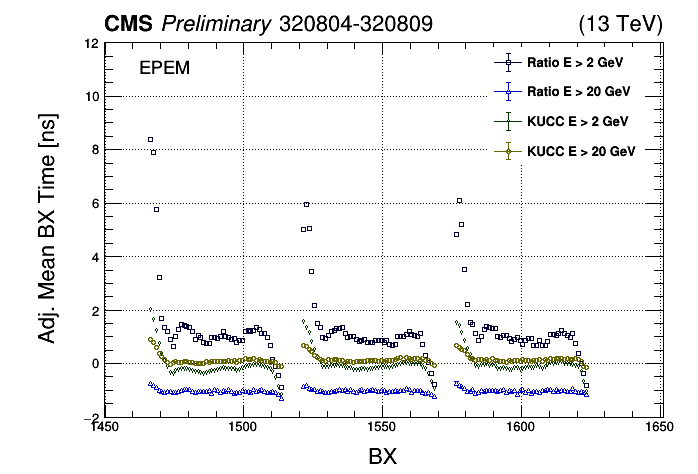
\includegraphics{fig/sec_results/tr_lhc_18A_v25_talk_30112021151421.png}}
\caption{Mean rechit time by BX for rechits with minimum energies of 2~GeV and 20~GeV, using both the ratio and CC reconstructions. Values are calibrated such that the mean time across all BXs and energies is zero. The CC algorithm mitigates OOT-PU effects, reducing BX dependence and energy dependence of the timing reconstruction.}
\label{cclhcplots1}
\end{center}
\end{figure}

Figure~\ref{cclhcplots1} demonstrates that the CC algorithm reduces the dependence of rechit time on BX position, particularly in the leading and trailing tails of the BX train. Additionally, the central regions show a reduced energy dependence for the CC method compared to the ratio method, highlighting its improved performance.

\begin{figure}[h!tbp]
\begin{center}
\resizebox{0.7\textwidth}{!}{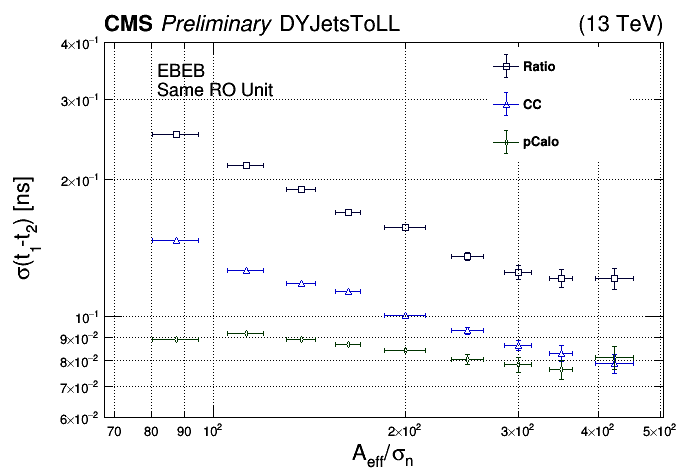
\includegraphics{fig/sec_gen/tr_mc_pc2_loc_plot_30112021153817.png}}
\caption{Single-crystal resolutions in simulation for the ratio algorithm, CC algorithm, and pCaloHit generator-level times. The CC algorithm significantly improves resolution relative to the ratio method and approaches the pCaloHit gen time at high energies.}
\label{pc_rt_cc_comp}
\end{center}
\end{figure}

During development, the CC algorithm was applied using a two-tier processing approach, allowing simultaneous comparison of CC and ratio reconstruction times. Studies in both simulation (MC) and recorded data confirm that the CC method improves timing performance.

\begin{figure}[h!tbp]
\begin{center}
\resizebox{0.7\textwidth}{!}{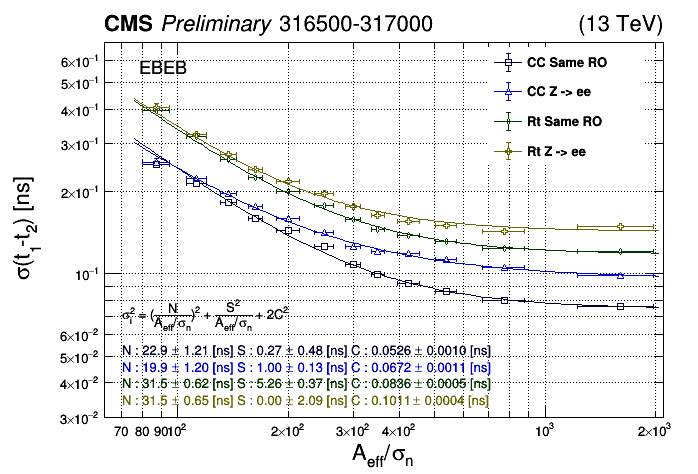
\includegraphics{fig/sec_results/tr_kucc_18As_v25_talk_30112021160215.png}}
\caption{Comparison of Same Readout (RO) unit and $Z\rightarrow e^{+}e^{-}$ resolutions in Run 2 for CC and ratio algorithms using two-tier processing and external calibrations. The CC algorithm achieves an improvement of approximately 30~ps in RO resolution and 35~ps in $Z\rightarrow e^{+}e^{-}$ resolution.}
\label{ccresr2}
\end{center}
\end{figure}

Figure~\ref{pc_rt_cc_comp} shows simulated single-crystal resolutions, indicating that the CC algorithm consistently outperforms the ratio algorithm and approaches the ideal pCaloHit generator-level resolution at high energies.

\begin{figure}[h!tbp]
\begin{center}
\resizebox{0.7\textwidth}{!}{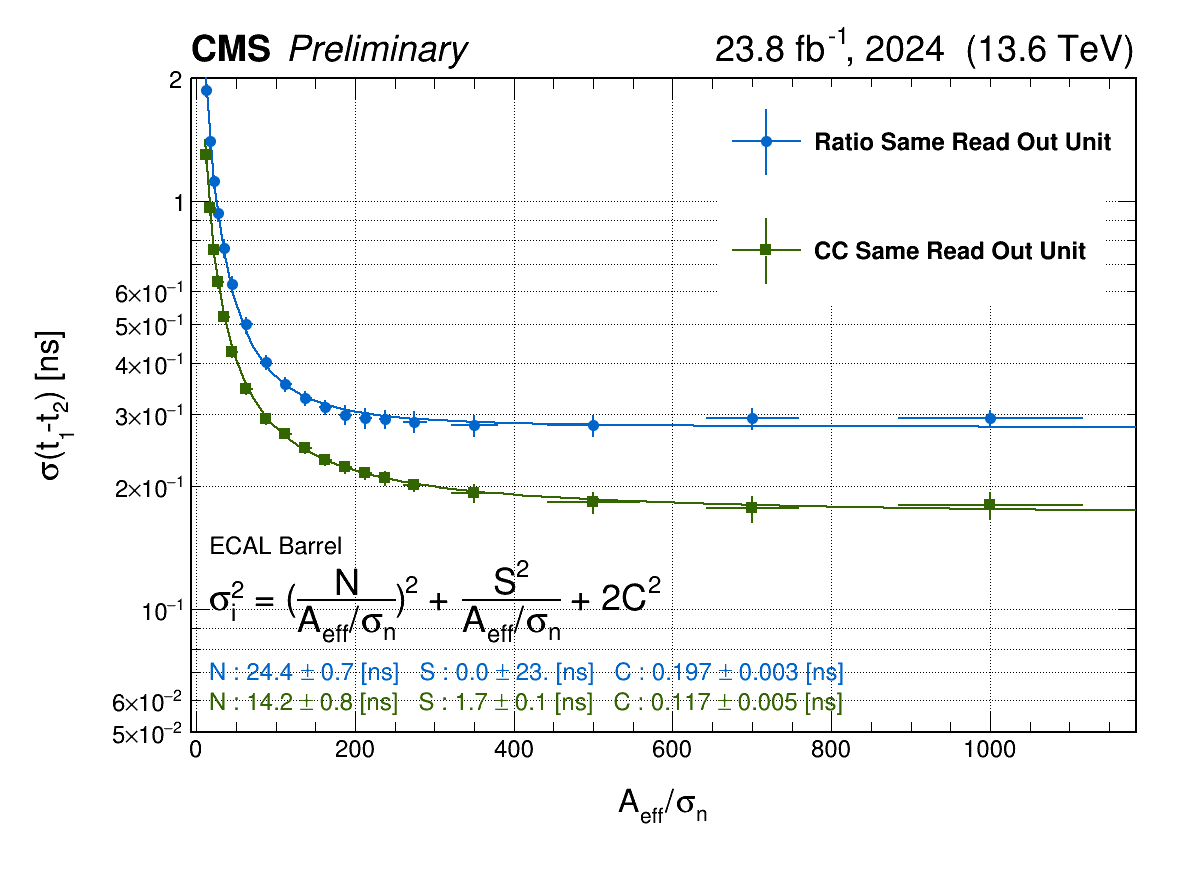
\includegraphics{fig/sec_results/tr_hl_r3_24f_v2_rtvcc_xgs_07082025170637.png}}
\caption{Same RO and $Z\rightarrow e^{+}e^{-}$ resolutions in Run 3. Comparative resolutions were obtained from two separate full prompt reconstructions using the ratio method and the CC method. The CC algorithm achieves an improvement of approximately 80~ps in RO resolution.}
\label{ccresr3}
\end{center}
\end{figure}

\begin{figure}[h!tbp]
\begin{center}
\resizebox{0.7\textwidth}{!}{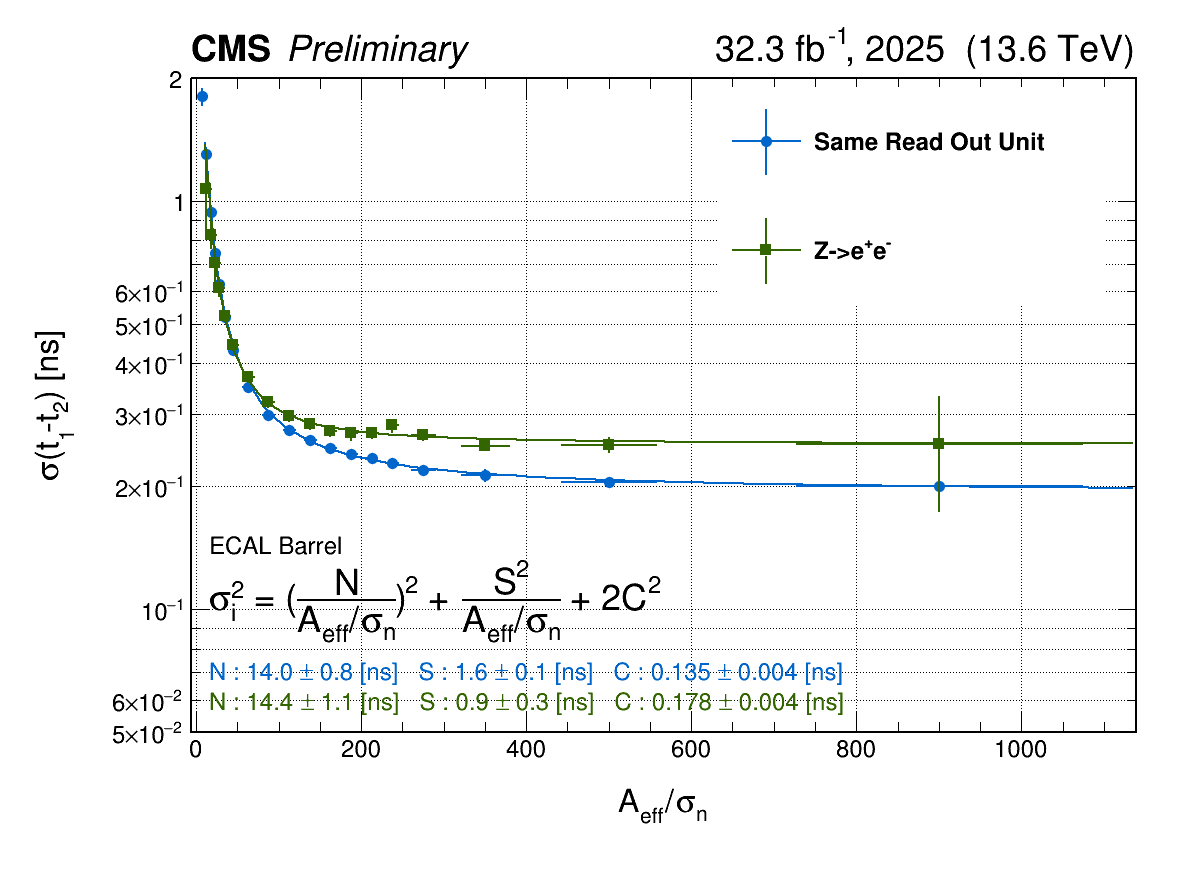
\includegraphics{fig/sec_results/tr_hl_r3_25c2_08082025165318.png}}
\caption{Same RO and $Z\rightarrow e^{+}e^{-}$ resolutions for the CC algorithm during Run 3 prompt reconstruction in 2025. The CC method achieves a RO resolution of approximately 135~ps and a $Z\rightarrow e^{+}e^{-}$ resolution of approximately 180~ps, demonstrating significant mitigation of OOT-PU effects.}
\label{ccresr4}
\end{center}
\end{figure}

These results demonstrate that the CC time reconstruction method consistently improves timing resolution across energy ranges and data-taking periods, both in simulation and recorded data, effectively reducing the impact of out-of-time pile-up.
